\documentclass{report}
\usepackage{polski}
\usepackage{tikz}
\usepackage{pgfplots}
\usepackage{amsmath}
 
\begin{document}

\date{Wrocław, \today}
\title{\LARGE\textbf{Zadanie z pierwszej pracowni}\\Analiza Numeryczna (M)}
\author{Bartosz Brzoza\thanks{\textit{E-mail}: \texttt{309426@ii.uni.wroc.pl}}}
\maketitle

\chapter{Sprawozdanie}
 
\section{Pierwszy dział}
 
To jest pierwszy dział.\\
Tutaj jest jakiś tekst.
 
\subsection{Poddział w pierwszym dziale}
 
Tu jest poddział.\\
Tutaj jest tabelka. \\
\begin{center}
    \begin{tabular}{||c c c c||} 
        \hline
        Lp. & Kategoria 1 & Kategoria 2 & Kategoria 3 \\ [0.5ex] 
        \hline\hline
        1 & 6 & 87837 & 787 \\ 
        \hline
        2 & 7 & 78 & 5415 \\
        \hline
        3 & 545 & 778 & 7507 \\
        \hline
        4 & 545 & 18744 & 7560 \\
        \hline
        5 & 88 & 788 & 6344 \\ [1ex] 
        \hline
    \end{tabular}
\end{center}
 
\section{Drugi dział}
 
To jest drugi dział.\\
Niech $Y$ będzie przestrzenią unormowaną oraz $f\colon [a,b]\to Y$ będzie funkcją $(n+1)$-razy różniczkowalną na 
przedziale $[a,b]$ w sposób ciągły (na końcach przedziału zakłada się różniczkowalność z lewej, bądź odpowiednio, 
z prawej strony). Wówczas dla każdego punktu $x$ z przedziału $(a,b)$ spełniony jest wzór zwany wzorem Taylora:
\begin{align}
$f(x) &= f(a) + \frac{x-a}{1!} f^{(1)}(a) + \frac{(x-a)^2}{2!} f^{(2)}(a) + \ldots + \frac{(x-a)^n}{n!} f^{(n)}(a) + R_n(x,a) = \sum\limits_{k=0}^n \left( \frac{(x-a)^k}{k!} f^{(k)}(a) \right) + R_n(x,a),$
\end{align}

gdzie $f^{(k)}(a)$ jest pochodną k-tego rzędu funkcji $f,$ obliczoną w punkcie $a;$ $R_n(x,a)$ spełnia warunek
: $\lim_{x\to a}\frac{R_n(x,a)}{(x-a)^n}=0$.
 
\subsection{Poddział w drugim dziale}
 
Tu jest kolejny poddział.\\
\begin{tikzpicture}
    \begin{axis}
    \addplot[color=red]{exp(x)};
    \end{axis}
    \end{tikzpicture}
    \hskip 5pt
    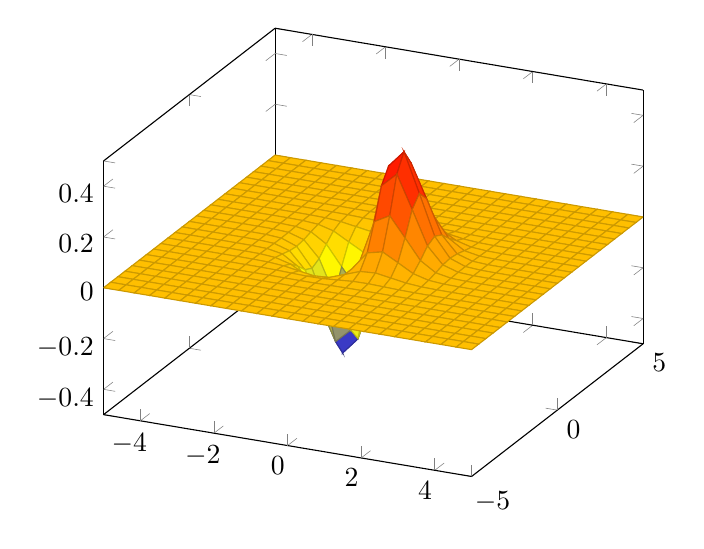
\begin{tikzpicture}
    \begin{axis}
    \addplot3[surf,]
    {exp(-x^2-y^2)*x};
    \end{axis}
\end{tikzpicture}
 
\end{document}